\documentclass[journal, a4paper]{IEEEtran}
\usepackage{graphicx} 
\usepackage{url}      
\usepackage{amsmath} 
 \begin{document}
	\title{Text Semantic Similarity - Group 3} 
	\author{Machine Learning Project - Mid Term Review
		\\Aneri Sheth (1401072)\\
		Himanshu Budhia (1401039)\\ Raj Shah (1401050)\\ Twinkle Vaghela (1401106) \\
		\vspace{1cm} }
	\maketitle
\begin{abstract}
Machine Learning has found its place in the technological world rapidly since the past few years. Text Semantic Similarity is one of the examples of Machine Learning with various applications in natural language processing,information retrieval and digital education. Text Semantic Similarity is a measure of the degree of semantic equivalence between two pieces of text. In this report, importance, limitations, approaches for text semantics and applications are discussed and results for comparing textual data in two files are shown. 
\end{abstract}
\begin{IEEEkeywords}
		Recursive Neural Networks, Recurrent Neural Networks, Optical Character Recognition (OCR), Machine Learning Algorithms
	\end{IEEEkeywords}
\section{Introduction}
	\PARstart{T}{he} fundamental challenge natural language processing or plagiarism checking softwares is to find out the meaning of text. Semantic similarity is important for various purposes - plagiarism checking, information retrieval and enabling machines to answer questions. But for machines, it is difficult to determine the semantics similarity. Due to advancement in Machine Learning, machines are getting better at Text Semantics and various algorithms are proposed. Semantic Analysis is not about teaching the machine, it is about getting them to learn. \\
	\begin{center}
	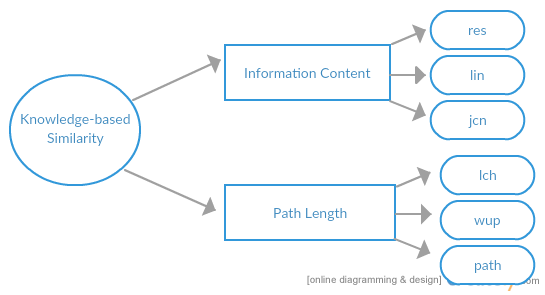
\includegraphics[width = 8cm,height = 6cm]{ML.png} \\
	\small Fig. 1 Block Diagram
	\end{center}
	
	The idea is to take two text files and then to separate the words in the sentences. Once the words are separated, the next step will be to find clues in the contextual data based on the data already there with the machine. For example, if the word 'happy' is encountered, then all the related words within the database will be searched to best match our data. Till now, the text semantic algorithms are considered and further research is going on. 
	
\section{Literature Review}
Text semantics has found its application in Information Retrieval, Plagiarism Checking, and many more. Text Semantic models in Information Retrieval are based on a bag-of-words representation of text, where large documents are simply represented as the frequency distribution of their terms. This representation disregards syntax or word order in the text and encodes only what topic the text is about. \\
Context of a token t in a given piece of text is defined as the set of tokens surrounding t within a pre-specified window size. Such distributional models represent a target word as a point in a vector space, derived from raw frequencies of its neighboring words or transformations such as dimensionality reduction applied to these frequencies. The latest generation of distributional models learn
word vectors that maximize the probability of observing each target word in its contexts in a large corpus. These word representations provide a much greater coverage than manually constructed lexical resources like WordNet. \\
Another major outcome is a rich literature for Semantics, describing around 300 systems that have been evaluated over a span of the years 2012$ - $2015. A vast majority of the best-performing systems at apply a regression algorithm that predicts similarity as a linear function of a wide array of text similarity measures. The methods include Semantic Overlap and n-gram overlap which are top-performing systems since the past few years. \\
There are Deep Learning Models like Recursive Neural Networks and Recurrent Neural Networks which also emerged as approached for text semantics. Recurrent Neural Network takes input as set of tokens which produces hidden vectors. Then we produce a vector whose values represent probability that the sentence pair belongs to the same category. The loss is calculated based on probability. Recurrent Neural Network is a powerful deep learning method.Recursive Neural Network takes input as a binary tree. The nodes of this tree represents the words in the sentence and we infer the binary tree using calculated parse of the sentence. The vector is calculated from the binary tree structure and the rest is similar as recurrent neural network. 

\section{Results}
\begin{center}
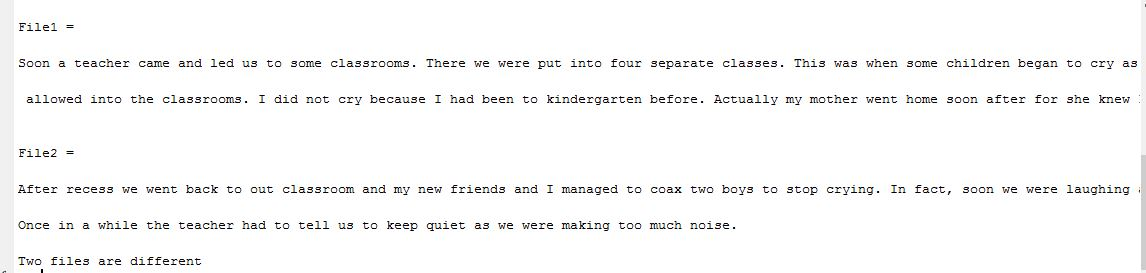
\includegraphics[width=7cm,height=4cm]{text_different.jpg} \\
\small Fig. 2 Text Comparison (For different text files)
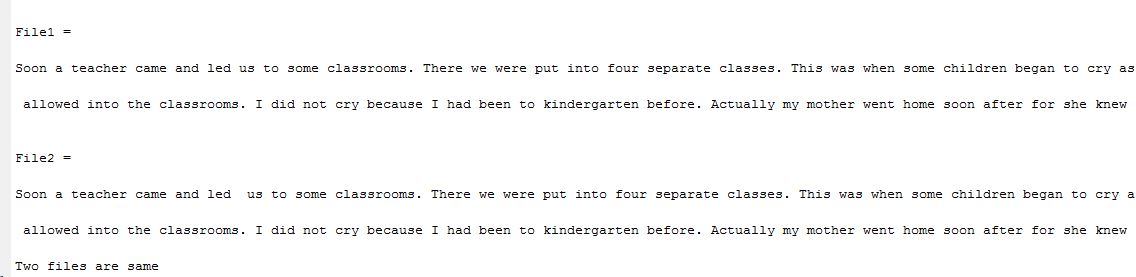
\includegraphics[width=7cm,height=4cm]{text_similarity.jpg} \\
\small Fig. 3 Text Comparison (For similar text files)
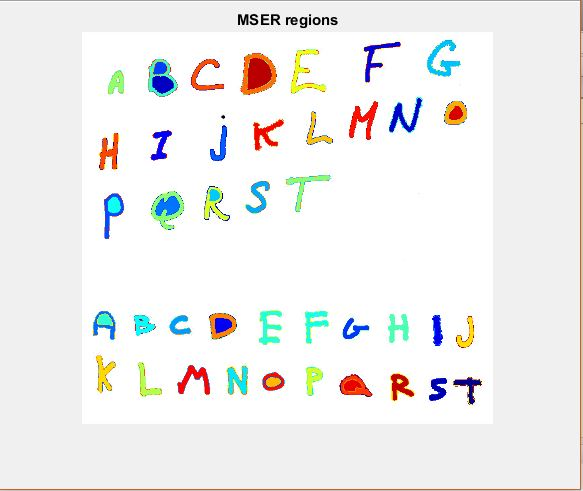
\includegraphics[width = 7cm , height = 5cm]{ocr_fig1.jpg} \\
\small Fig 4. OCR  MSER Regions 
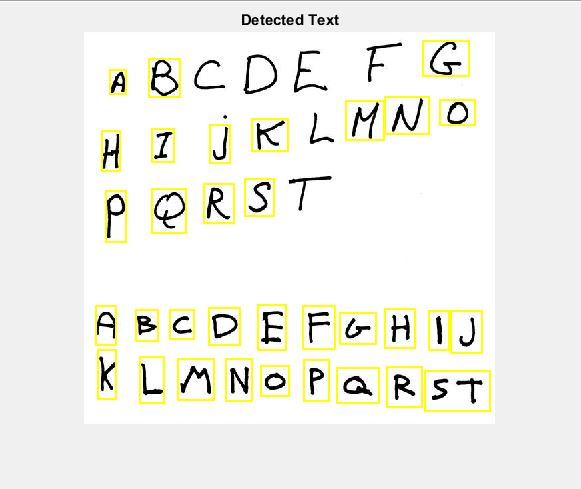
\includegraphics[width = 7cm , height = 5cm]{ocr_fig6.jpg} \\
\small Fig 5. OCR Detected Text 
\end{center}
This section includes the results and simulation that are generated in MATLAB. Text Semantics Similarity can be done either on text files (part of Natural Language Processing ) or the text can be compared from images (like Optical Character Recognition).
\begin{itemize}
\item Comparing two text files (MATLAB Simulation) - From the output above [Fig. 2 and 3], we see that by taking two input text files and separating the space (a delimiter) between the characters, we can compare the characters. 
\item Two images having textual data can also be compared. This is done using OCR (Optical Character Recognition) . This algorithm was explored for comparing text semantics from PDFs (in this case, the input will be images) [Fig. 4 and 5]. 
\end{itemize}


\section{Discussion}
As a part of Machine Learning Course, the project 'Text Semantic Similarity' we will be able to show the results for comparing the text files by finding the meaning of those sentences in the text files. 
By looking at the two results above, we have understood the basic steps and approaches on how Text Semantics Similarity will work. But we still have to decide upon the algorithms. What we will possibly do is try out different algorithms and compare the performance of those. 
\section{Future Work}
By the end of the final project review, we as a team of 4 with mentoring by Prof. Mehul Raval and our teaching assistant Shashwat Sanghavi intend to show the following results which in this report is included as a part of future work. 
\begin{itemize}
\item Implement Text Semantic Similarity algorithm. (one or more)
\item Try out different algorithms and compare them with our implemented algorithm.
\item Literature Study of papers, thesis and related articles.
\item Demonstrate the semantics algorithm for applications like Plagiarism Checking. 
\end{itemize}
\begin{thebibliography}{5}
\bibitem{1} T.  graph, "Text semantic analysis and semantic graph", Stackoverflow.com, 2017. [Online]. 
Available: http://stackoverflow.com/questions/35666726/text-semantic-analysis-and-semantic-graph. [Accessed: 27- Feb- 2017].

\bibitem{2} "How to do Semantic Keyword Research Using NLP and Text Analysis - AYLIEN", AYLIEN, 2017. [Online].
Available: http://blog.aylien.com/how-to-do-semantic-keyword-research-using-nlp-and/. [Accessed: 01- Mar- 2017].

\bibitem{3}"Understanding Semantic Analysis (And Why This Title is Totally Meta) - Boomtrain", Boomtrain, 2017. [Online].
Available: https://boomtrain.com/understanding-semantic-analysis/. [Accessed: 01- Mar- 2017].

\bibitem{4}[Online]. Available: https://cs224d.stanford.edu/reports/SanbornAdrian.pdf. [Accessed: 05- Mar- 2017].

\bibitem{5}[Online]. Available: http://nlp.stanford.edu/pubs/wordwalk-textgraphs09.pdf. [Accessed: 02- Mar- 2017].

\bibitem{6}"How does OCR document scanning work?", Explain that Stuff, 2017. [Online]. 
Available: http://www.explainthatstuff.com/how-ocr-works.html. [Accessed: 15- Feb- 2017].

\bibitem{7}"Image Processing in MATLAB Tutorial 6: OCR in Natural Images", YouTube, 2017. [Online].
Available: https://www.youtube.com/watch?v=JJLDOO4Xh8Y. [Accessed: 24- Feb- 2017].

\bibitem{8}"Maximally stable extremal regions", En.wikipedia.org, 2017. [Online]. 
Available: https://en.wikipedia.org/wiki/Maximallystableextremalregions. [Accessed: 26- Feb- 2017].

\end{thebibliography}
\end{document}
